\section{Documentación de la librería}

\subsection{Desarrollo de la documentación}

Para esto se utiliza el paquete sphinx de Python \url{http://www.sphinx-doc.org} y el tema Read The Docs \url{https://readthedocs.org}.

La selección de estas herramienta se debe a que permite generar documentación automáticamente a través de comentarios en el código, lo que facilita en gran medida esta tarea

\subsection{Ejemplos de la documentación}

La pagina inicial de la librería puede verse en la figura  \ref{fig:lamfriaA}

\begin{figure}[H]
    \centering
    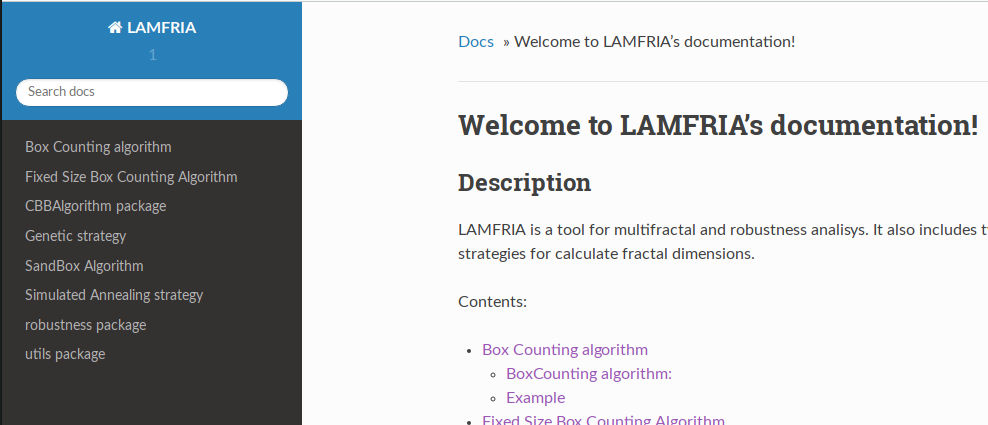
\includegraphics[scale=0.45]{Capitulo7Libreria/imagenes/lamfriaA.png}
    \caption{Pagina inicial de la documentación de la librería}
    \label{fig:lamfriaA}
\end{figure}

Al hacer clic en alguna de las funciones del menú izquierdo, se puede ampliar la información:


\begin{figure}[H]
    \centering
    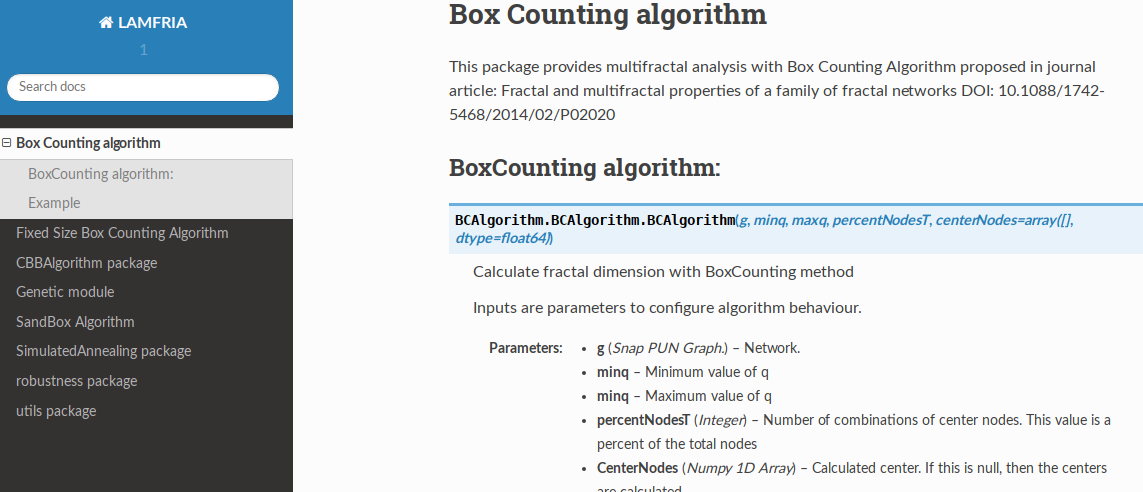
\includegraphics[scale=0.4]{Capitulo7Libreria/imagenes/lamfriaB.png}
    \caption{Información especifica sobre una función de la librería}
    \label{fig:lamfriaB}
\end{figure}

Así mismo, se puede hacer búsqueda de información dentro de la documentación, en este caso la palabra \textit{genetic}

\begin{figure}[H]
    \centering
    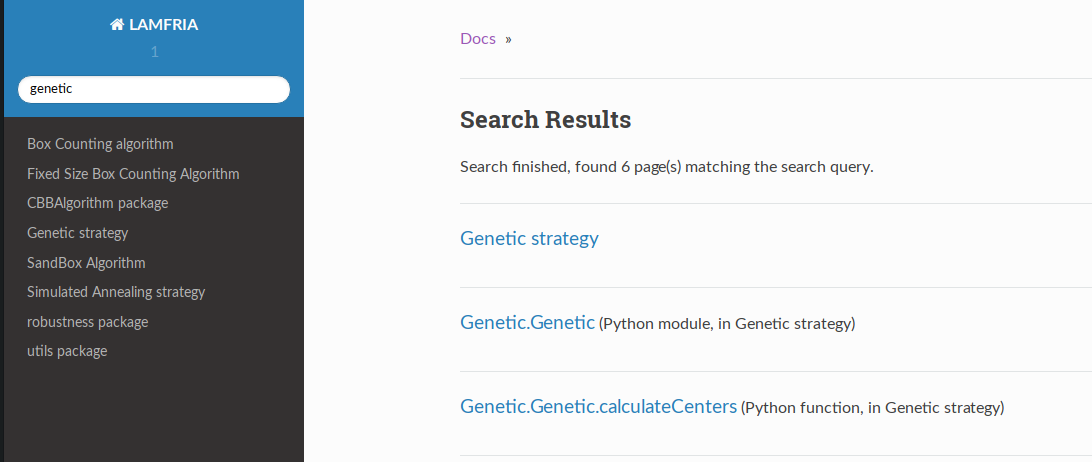
\includegraphics[scale=0.45]{Capitulo7Libreria/imagenes/lamfriaC.png}
    \caption{Resultado búsqueda información de la documentación en de la librería}
    \label{fig:lamfriaC}
\end{figure}